\documentclass{article}

\usepackage{tikz}

\begin{document}
\pagestyle{empty}

\resizebox{0.95\linewidth}{!}{%
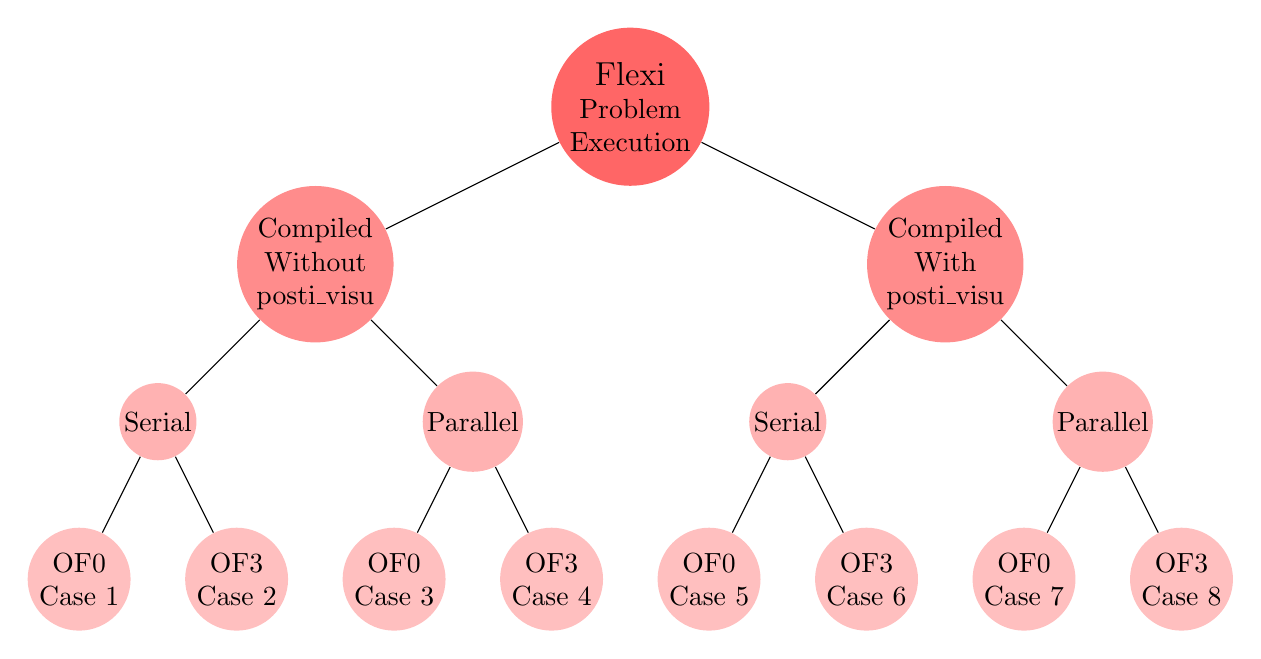
\begin{tikzpicture}
 [level distance=2cm,
   every node/.style={fill=red!60,circle,inner sep=1pt},
   level 1/.style={sibling distance=8cm,nodes={fill=red!45}},
   level 2/.style={sibling distance=4cm,nodes={fill=red!30}},
   level 3/.style={sibling distance=2cm,nodes={fill=red!25}}]
  \node[align=center] {\large Flexi \\  Problem \\ Execution}
     child {node[align=center] {Compiled \\ Without \\ posti\_visu}
       child {node {Serial}
         child[align=center] {node {OF0 \\ Case 1}}
         child[align=center] {node {OF3 \\ Case 2}}
       }
       child {node {Parallel}
         child[align=center] {node {OF0 \\ Case 3}}
         child[align=center] {node {OF3 \\ Case 4}}
       }
     }
     child {node[align=center] {Compiled \\ With \\ posti\_visu}
       child {node {Serial}
         child[align=center] {node {OF0 \\ Case 5}}
         child[align=center] {node {OF3 \\ Case 6}}
       }
       child {node {Parallel}
         child[align=center] {node {OF0 \\ Case 7}}
         child[align=center] {node {OF3 \\ Case 8}}
         }
     };
\end{tikzpicture}
}
\end{document}
